\section{Meiser's Algorithm}

Since the beginning of this writing, we were only interested by the number of
questions we ask to an oracle, and we will continue to take the same point of
view here. We wonder how many times we need to ask an oracle whether a point
lies above, on or under a certain hyperplane.

Given a set of hyperplanes \(\H\) and an input vertex \(x\) in \(\R^n\),
Meiser's algorithm \cite{meiser:1993} determines the position vector\footnote{
For this section, notation is strongly inspired by the notation
used for the detailed explanation of the same problem in \citet*{burgisser:1997}.
The relevant section from this reference is numbered \textbf{3.4} and titled
\emph{Fast Point Location in Arrangement of Hyperplanes}.
}
$\pv(x) \in
\signset^{m}$ of $x$ inside the
arrangement of hyperplanes $\arrangement(\H)$.
We show how to solve \kSUM using \BigO{k n^3 \log^3 n} $n$-variate
linear queries with this algorithm.

For \(k\) fixed,
\(\H\) is the set of hyperplanes having equation involving exactly $k$
coordinates of $\R^n$ with coefficient $1$, we have thus $\card{\H} = m =
\binom{n}{k}$. We can do this without involving the input vertex at all, this
costs us $0$ queries.

We give each hyperplane an orientation so that when the point $x$ is below
the
hyperplane $H_i$, it is in the lower half-space defined by $H_i$ denoted
$\Him$. When the point $x$ is above the hyperplane $H_i$ it is in the upper
half-space defined by $H_i$ denoted $\Hip$. We define $\Hiz$ to be the
hyperplane $H_i$ itself. The $i^{th}$ component of the position vector is
$\pv_i(x) = \sigma$ if and only if $x \in \His$.

Our first idea to determine the components of $\pv(x)$ is to iteratively
select a random subset of hyperplanes \(\Ht\) of size \BigO{\poly(n)}
for which the relative position of $x$ is not
determined yet. Once we have
computed the position vector of \(x\) for this subset \(\Ht\)
we have effectively determined in
which cell\footnote{Note that we always consider that \(x\) is inside a cell that is bounded.
This can be implicitly or explicitly simulated.}
of the arrangement $\arrangement(\Ht)$ $x$ lies.

We are left with hyperplanes of the set $\H \setminus \Ht$. They can be
partitioned in two disjoint sets: a set $\M$ of hyperplanes that meet the cell of
$\Ht$ containing $x$ and a set $\O$ for the others. The relative position of $x$
to each hyperplane belonging to $\O$ can be deduced without the need to query
the oracle, the answer to the queries we would make can be computed by looking
at the structure of the arrangement. For the first group of hyperplanes
we call the procedure again with $\H \gets \M$.

If we stop our explanation here we still have a worst-case \BigO{m}
bound on the number of queries made. Hopefully, the next step of our
explanation shows that it is possible to lower this bound.

The problem we have with our current algorithm is that there is no guarantee
on the number of queries we avoid at each step.
We use a result on \enets, attributed to Ken Clarkson by
\citet{burgisser:1997}, to make our algorithm achieve an upper bound
of \BigO{n^3 \log^2 n \log m} queries.
\begin{theorem}[Clarkson]\label{thm:meiser:clarkson}
Given a set $\H$ of $m$ hyperplanes in $\R^n$ and $\epsilon$ with the
constraint that $0 < \epsilon < 1$, there exists a subset $\NH \subseteq \H$ of
size $\BigO{\enetsize}$ such that for every simplex $\simplex$ in $\R^n$, if the
number of hyperplanes of $\H$ intersecting $\simplex$ is strictly greater than
$\epsilon \card{\H}$ then at least one of them belongs to $\NH$.
\end{theorem}

By applying a theorem due to \citet*{haussler:1987},
\citet{burgisser:1997} also prove (in addition to \ref{thm:meiser:clarkson}) that it is possible to
construct $\NH$ with high probability using a random uniform sampling on $\H$,
meaning the following corollary holds
\begin{corollary}
If we choose $\BigO{\enetsize}$ hyperplanes uniformly at
random from our $m$ hyperplanes and denote this selection $\H^{*}$ then for
any simplex intersected by more than $\epsilon \card{\H}$ hyperplanes of $\H$
there is a high probability that at least one of them is contained in $\H^{*}$.
\end{corollary}

If we take the contraposition of this corollary we obtain the following one
\begin{corollary}
If there is no hyperplane in $\H^{*}$ intersecting a given simplex, then, with
high probability, the number of hyperplanes of $\H$ intersecting the simplex
is less or equal to $\epsilon \card{\H}$.
\end{corollary}

We can use this corollary in the algorithm we were describing earlier. We
make two changes to the previous algorithm, we explicitly define the
cardinality of $\Ht$ and we include an additional step where we replace cell
$\cell$ with a simplex $\simplex$.

Remember \(\Ht\) is the set of hyperplanes for which we query the oracle
in the current step of the algorithm. We choose \(\card{\Ht} = \BigO{\enetsize}\) and
instead of discarding hyperplanes not meeting the cell $\cell$ of the
arrangement $\arrangement(\Ht)$ containing $x$, we first refine the cell around
point $x$. We do so by computing a simplex $\simplex$ inscribed in $\cell$ and
containing \(x\). Then we discard hyperplanes that do not meet this simplex.

By proceeding this way we have the guarantee that we keep at most a
constant fraction \(\epsilon\) of the hyperplanes and thus the total number of
queries made to determine the enclosing cell of
all steps is \BigO{n^2 \log^2 n \log m}. However, we
still need to explicit how we find a simplex $\simplex$ containing $x$ and
inscribed in $\cell$.

We explain how to build $\simplex$. The algorithm can be sketched as
follows
\begin{algorithm}[Building \(\simplex\)]
\item[input] A point \(x\) and a set of hyperplanes \(\widetilde{\H}\) in
\(\R^n\).
\item[1.] Find a vertex $\nu$ of the cell containing $x$, $\nu$ is one of
the vertices of our simplex.
\item[2.] Compute $x'$, the projection of $x$ along $\vec{\nu x}$ on the
boundary of \(\cell\).
\item[3.] Let \(H_{\theta}\) denote the hyperplane in \(\widetilde{\H}\)
containing \(x'\). Compute \(\widetilde{\H}'\) as the intersection of all
hyperplanes of \(\widetilde{\H} \setminus \enum{H_{\theta}}\) with
\(H_{\theta}\).
\item[4.] Induction on \(x'\) and \(\widetilde{\H}'\) in $\R^{n-1}$, store result in \(\simplex'\).
\item[5.] Return \(\simplex\), the convex hull of \(\simplex' \cup \enum{\nu}\).
\end{algorithm}

We can solve step \step{1} by using linear programming with our \BigO{n^2
\log^2 n} hyperplanes and the answers to queries $x \ask{\in} \His, \sigma \in
\signset$ as constraints of the linear program. We arbitrarily choose an
objective function with a gradient non-orthogonal to all hyperplanes in
\(\widetilde{\H}\) and look for
the optimal solution. The optimal solution being the intersection of \(n\)
hyperplanes from the arrangement, its coordinates are independent of the exact
location of \(x\) inside its cell and thus this step involves no query at all.

In step \step{2} we find the projection of $x$ on one of the faces of
$\cell$ by computing the closest hyperplane of $\Ht$ to $x$ in direction
$\vec{\nu x}$. This is done by projecting $x$ on every hyperplane of $\Ht$ and
then computing the distance between $x$ and his projections, keeping the
projection that is the closest in the correct direction as the projection
on $\cell$. Each such projection and distance computation counts as one query
since this computation could be used to forge a query. The number of
projections to compute is \(\card{\Ht}\) and hence the query complexity of this
step is $\BigO{\enetsize}$.

Step \step{3} prepares the induction step by computing the arrangement of
hyperplanes \(\A(\widetilde{H}')\) in \(\R^{n-1}\). Like step \step{1}, this
computation does not involve the input point \(x\) and therefore uses no query.

In step \step{4} the base case is $n = 0$. In $\R^0$ we have only one point
and this point is the last vertex of our simplex.
The recursion depth is $n$, the dimension of $R^n$, and thus the total number
of queries made to compute $\simplex$ is \BigO{n^3 \log^2 n}.

Remember that once we have the simplex $\simplex$, we do not need to query the
input point $x$ to sort out which hyperplanes meet $\simplex$. The simplex is
composed entirely of vertices and faces from the hyperplane arrangement
$\arrangement(\Ht)$. Hence, its structure does not depend on $x$.

\begin{figure}
\begin{center}
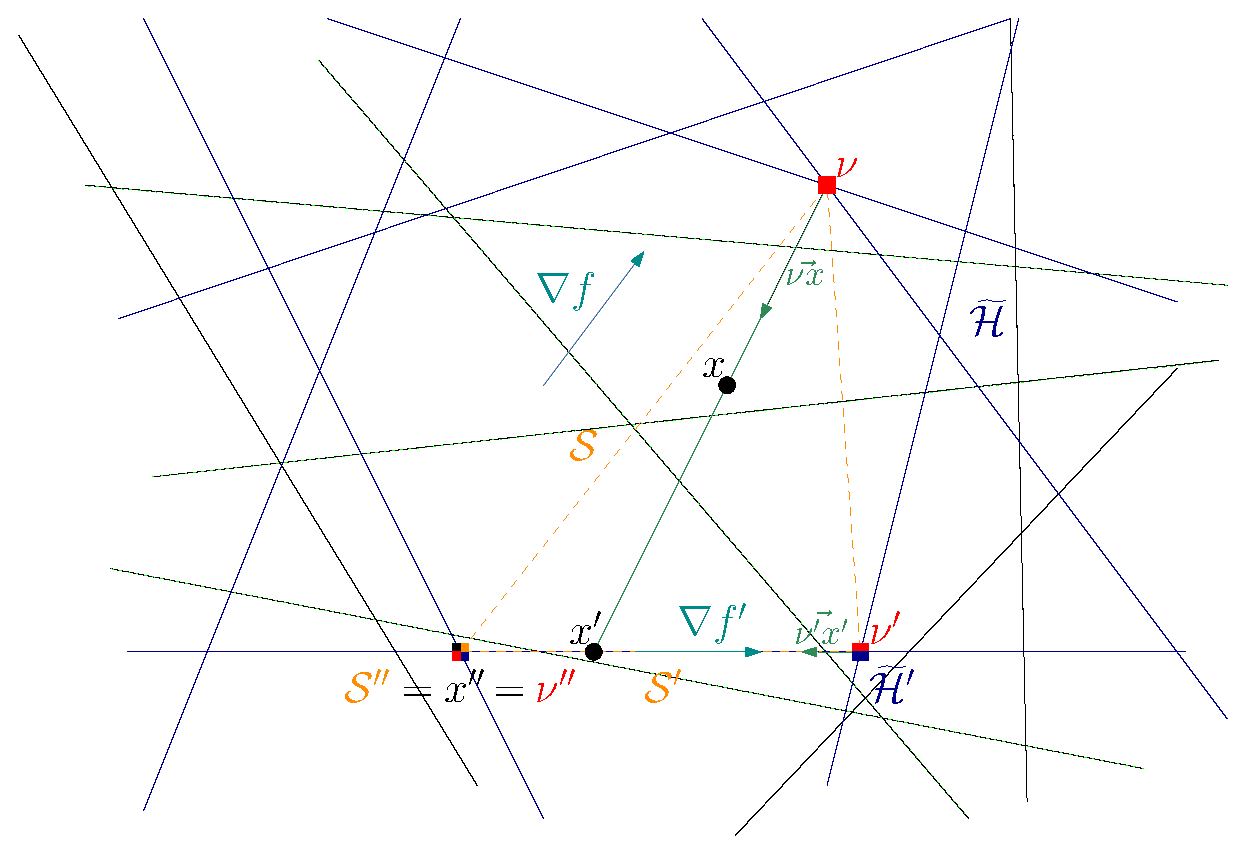
\includegraphics[trim=110 40 50 30,clip=true,height=0.3\textheight]{fig/point-location/simplex.eps}
\caption{
A complete step of Meiser's algorithm. The blue lines are hyperplanes of the
set \(\widetilde{\H}\). The gradient of the objective function
chosen to find the first vertex of the simplex is \(\nabla f\). The green dotted lines are the
hyperplanes from \(\H \setminus \widetilde{\H}\) that meet \(\S\), those are
the only hyperplanes that are left to process after this step.
}
\label{fig:meiser:step}
\end{center}
\end{figure}

\ref{fig:meiser:step} shows a complete step of Meiser's algorithm.
Let us summarize the algorithm
\begin{algorithm}[Meiser's algorithm]
\item[input] $x \in \R^n$, the point to be located.
\item[1.] Compute the position of $\BigO{n^2 \log^2 n}$ hyperplanes relatively to
$x$, effectively computing cell $\cell$ containing $x$.
\item[2.] Recursively build simplex $\simplex$ containing $x$ and inscribed in
$\cell$.
\item[3.] For any hyperplane $H_i$ not meeting the simplex, deduce $\pv_i(x)$.
\item[4.] Discard all hyperplanes that do not meet the inside of the
simplex.
\item[5.] Recurse on hyperplanes that are left.
\end{algorithm}

Since the complexity of step \step{1} is \BigO{n^2 \log^2 n}, the complexity of step
\step{2} is \BigO{n^3 \log^2 n}, the complexity of steps \step{3} and \step{4}
is \(0\),
and the induction depth is $\BigO{\log m}$, the total complexity of this algorithm
is \BigO{n^3 \log^2 n \log m}. For our \kSUM problem, $m = \binom{n}{k}$,
and thus the complexity is \BigO{k n^3 \log^3 n}. Note that the overall
complexity in the Random Access Machine model is polynomial.

In the next section we apply the same algorithm to solve the
subset sum problem and show that in our sufficiently powerful computing
model the subset sum problem has polynomial complexity.

